
\section*{Verkaveling}

Bij een verkaveling wordt een stuk land opgedeeld in verschillende kavels die elk een andere eigenaar kunnen hebben. Vroeger hadden de boeren kleine stukken land, die vaak door elkaar heen lagen. Een boer moest toen over het land van een andere boer lopen of rijden om naar zijn eigen kavels te gaan. Tengevolge van de schaalvergroting van de landbouw wordt tegenwoordig gewerkt met vierkante kavels, en streven boeren ernaar om te werken met zo groot mogelijke percelen: rechthoekige gebieden van aaneengesloten kavels.

Onderstaand voorbeeld toont een rechthoekig stuk land dat werd opgedeeld in $10 \times 10$ vierkante kavels. Drie percelen (witte rechthoeken) werden reeds door boeren in gebruik genomen. Zoek de oppervlakte van het grootst mogelijke perceel waarvan nog geen enkel kavel in gebruik werd genomen. In dit voorbeeld is dit een perceel dat bestaat uit 16 kavels, zoals aangegeven door de gestreepte rechthoek.

\begin{figure}[H]
  \begin{center}
    \centerline{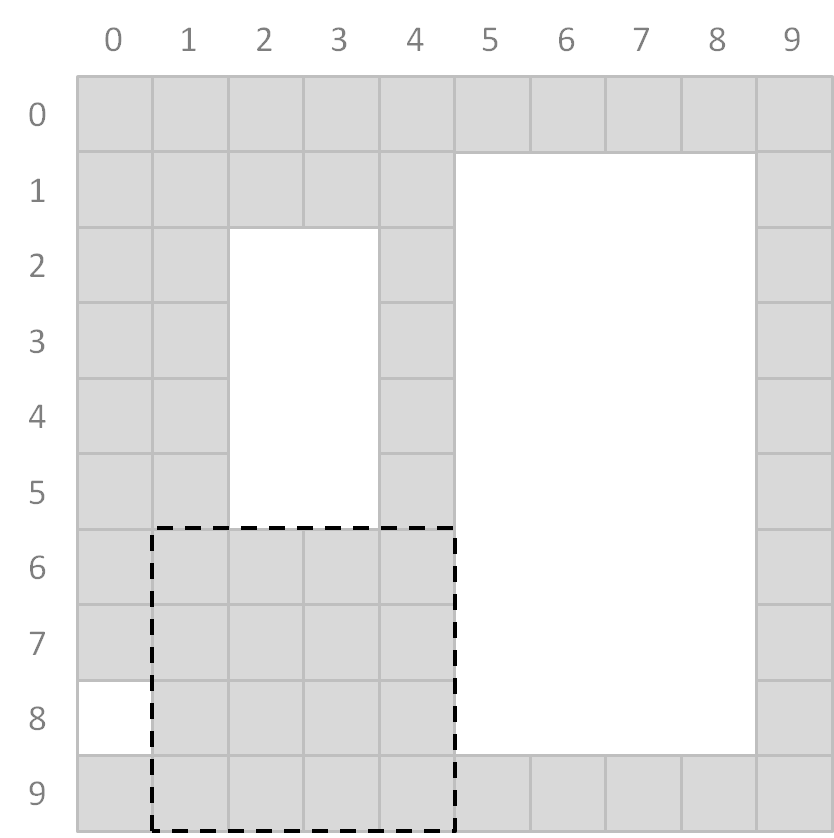
\includegraphics[scale=0.30]{verkaveling/verkaveling.png}}
  \end{center}
\end{figure}

\subsection*{Input}
\subsubsection*{Voorbeeldinput}
\begin{verbatim}
2
8 12
############
############
############
############
############
############
############
############
8 12
############
############
############
#####--#####
#####--#####
############
############
############
\end{verbatim}
\subsection*{Output}
\subsubsection*{Voorbeeldoutput}
\begin{verbatim}
96
40
\end{verbatim}

\end{itemize}